%%%%
% -- Galaxies Science Cases
% --     FOBOS Keck White Paper 2019
%%%%

\subsection{A Comprehensive Picture of the Proto-galaxy Ecosystem}
\label{sec:galaxies}

% From George:
% - fill out case for probing both galaxies and their “gas-filled
%   environments”
%    - make it more explicit that getting large numbers of redshifts
%      would make it possible to trace out large-scale structure in
%      detail
%    - enables studies of galaxy properties as a function of environment
%
% - also mention targeting galaxies along QSO lines of sight
%    - much higher target density than with LRIS, DEIMOS over larger FOV.
%
% - Worth discussing Lyman-alpha or metal-line tomography?  
%
% - More quantitative comparisons with existing data sets?
%    - What key science questions can FOBOS address that many years of
%      LRIS and DEIMOS observations have not been able to?  Surely some
%      level of the spectral tagging and photo-z training can be done
%      (and surely is being done) with existing data.  Is FOBOS going to
%      be a huge leap, or will it mainly be cleaning up neglected corners
%      of parameter space?
%
% - More excited to hear about how the FOBOS spectra will be used for
%   science directly, instead of support for LSST

Roughly three billion years after the Big Bang ($z$$\sim$2), the universe began a key epoch in which proto-galaxies
transitioned from turbulent, gas-rich systems into the more ordered, star-dominated structures that populate the
universe today.  This period marks the peak of cosmic star formation and galaxy assembly.   To understand it, we must
study the entire galaxy ``ecosystem,'' including not only the galaxies themselves but their gas-filled environments.
The goal is to build a comprehensive picture of the physical processes that fuel proto-galaxy growth, shape their
internal structure, and influence their environment.

Although our first challenge emphasized photo-$z$ training, here we will apply machine learning more broadly to infer
physical parameters from multi-wavelength photometry as well as lower quality spectra trained with high-S/N data sets 
(cf., Fig.~\ref{fig:absorber}).  Given the cost of deep spectroscopy, a central goal is to extract the maximum
information from photometry and shallower spectroscopy so that more statistically powerful samples over larger cosmic
volumes can be studied.

%  build SDSS-like
% statistics for galaxies at this key cosmic epoch.  In all of these
% challenges, we will use simulated data sets to isolate uncertainties and
% biases in various training-set design strategies, including the benefits
% of additional imaging information like morphology and size from a wide
% range of wave-bands (e.g., combining LSST, Euclid, WFIRST).  The
% exercise will define requirements for FOBOS instrument performance and
% the optimal training sample delivered publicly.

% LSST's panoramic imaging will detect huge numbers of galaxies at this
% epoch.  Targeted followup with FOBOS will allow us to ascribe detailed
% galaxy and environmental information from deep spectroscopic training
% samples to the much larger cosmic volumes surveyed with broad-band
% imaging.

\begin{enumerate}[rightmargin=0.2cm,leftmargin=0.2cm]
%
\chal{phot}
%
\item[] {\textsf {\large Data-Science Challenge \ref{phot}: Apply deep-
learning algorithms to infer physical properties of galaxies at
$z$$\sim$2 using using photometry.}} The range of observed spectral
types is well-constrained by broad-band imaging (Figure \ref{fig:SOM}),
suggesting a far greater potential for imaging data to reveal physical
properties with sufficient training than conventional modeling of
spectral energy distributions (SEDs) would suggest.  The challenge here is to identify the extent to which machine
learning can deliver SDSS-like information --- e.g., star-formation histories,
stellar-population properties, dust content, inflow/outflow properties,
and stellar masses --- and determine design parameters for future training sets that will enable such inferences for millions of imaged galaxies at $z$$\sim$2.
%
\end{enumerate}

% \begin{enumerate}[rightmargin=0.2cm,leftmargin=0.2cm]
% %
% \chal{uv}
% %
% \item[] {\textsf {\large Data-Science Challenge \ref{uv}: Infer stellar
% and ISM indicators in UV spectra from rest-frame optical spectra}}.
% There are many powerful gas and stellar spectral features just redward
% of the Lyman-$\alpha$ line at 1216\AA.  By combining FOBOS UV and
% existing near-IR spectroscopy at $z$$\sim$2, we can transfer physical
% ``labels'' determined in the rest-frame optical to spectra at UV
% wavelengths, which will dramatically enhance interpretation of JWST
% discoveries of the first galaxies ($z$$\sim$10) for which rest-frame UV
% imaging and spectroscopy will be most accessible.  A similar application
% can ascribe the escape fraction of Lyman-continuum radiation observed in
% FOBOS spectra to constrain the sources responsible for ``reionization''
% at $z$$\sim$6 \citep[cf.]{2018ApJ...869..123S}.

% % With simulated spectral observations, we will determine the extent of
% % label transfer that is possible and set requirements on training
% % samples.

% \end{enumerate}

\begin{enumerate}[rightmargin=0.2cm,leftmargin=0.2cm]
%
\chal{lowsnr}
%
\item[] {\textsf {\large Data-Science Challenge \ref{lowsnr}: Train
short spectroscopic exposures in combination with photometry to provide
environmental diagnostics for 1M galaxies at $z$=1--2}}.  Photometric
redshifts, while acceptable in large cosmological analyses, wash out
information about the local position of galaxies with respect to one
another.  To characterize a galaxy's local environment and identify its
neighbors requires (observationally expensive) spectroscopic redshifts.  However, with improved photo-$z$s available
from Challenge \ref{photozs} and strong priors on spectral types
(Challenge \ref{phot}), the challenge here is to push machine-learning techniques to deliver
\emph{spectroscopic} redshifts (with 300 km s$^{-1}$ accuracy) at the lowest signal-to-noise possible.  Reductions by
factors of 4--5 in exposure time would enable FOBOS to complete a 1M galaxy environment survey at $z=1$--$2$ in just
20-30 nights.

\end{enumerate}

\begin{figure}[h!]
%
\vskip -0.1in
%
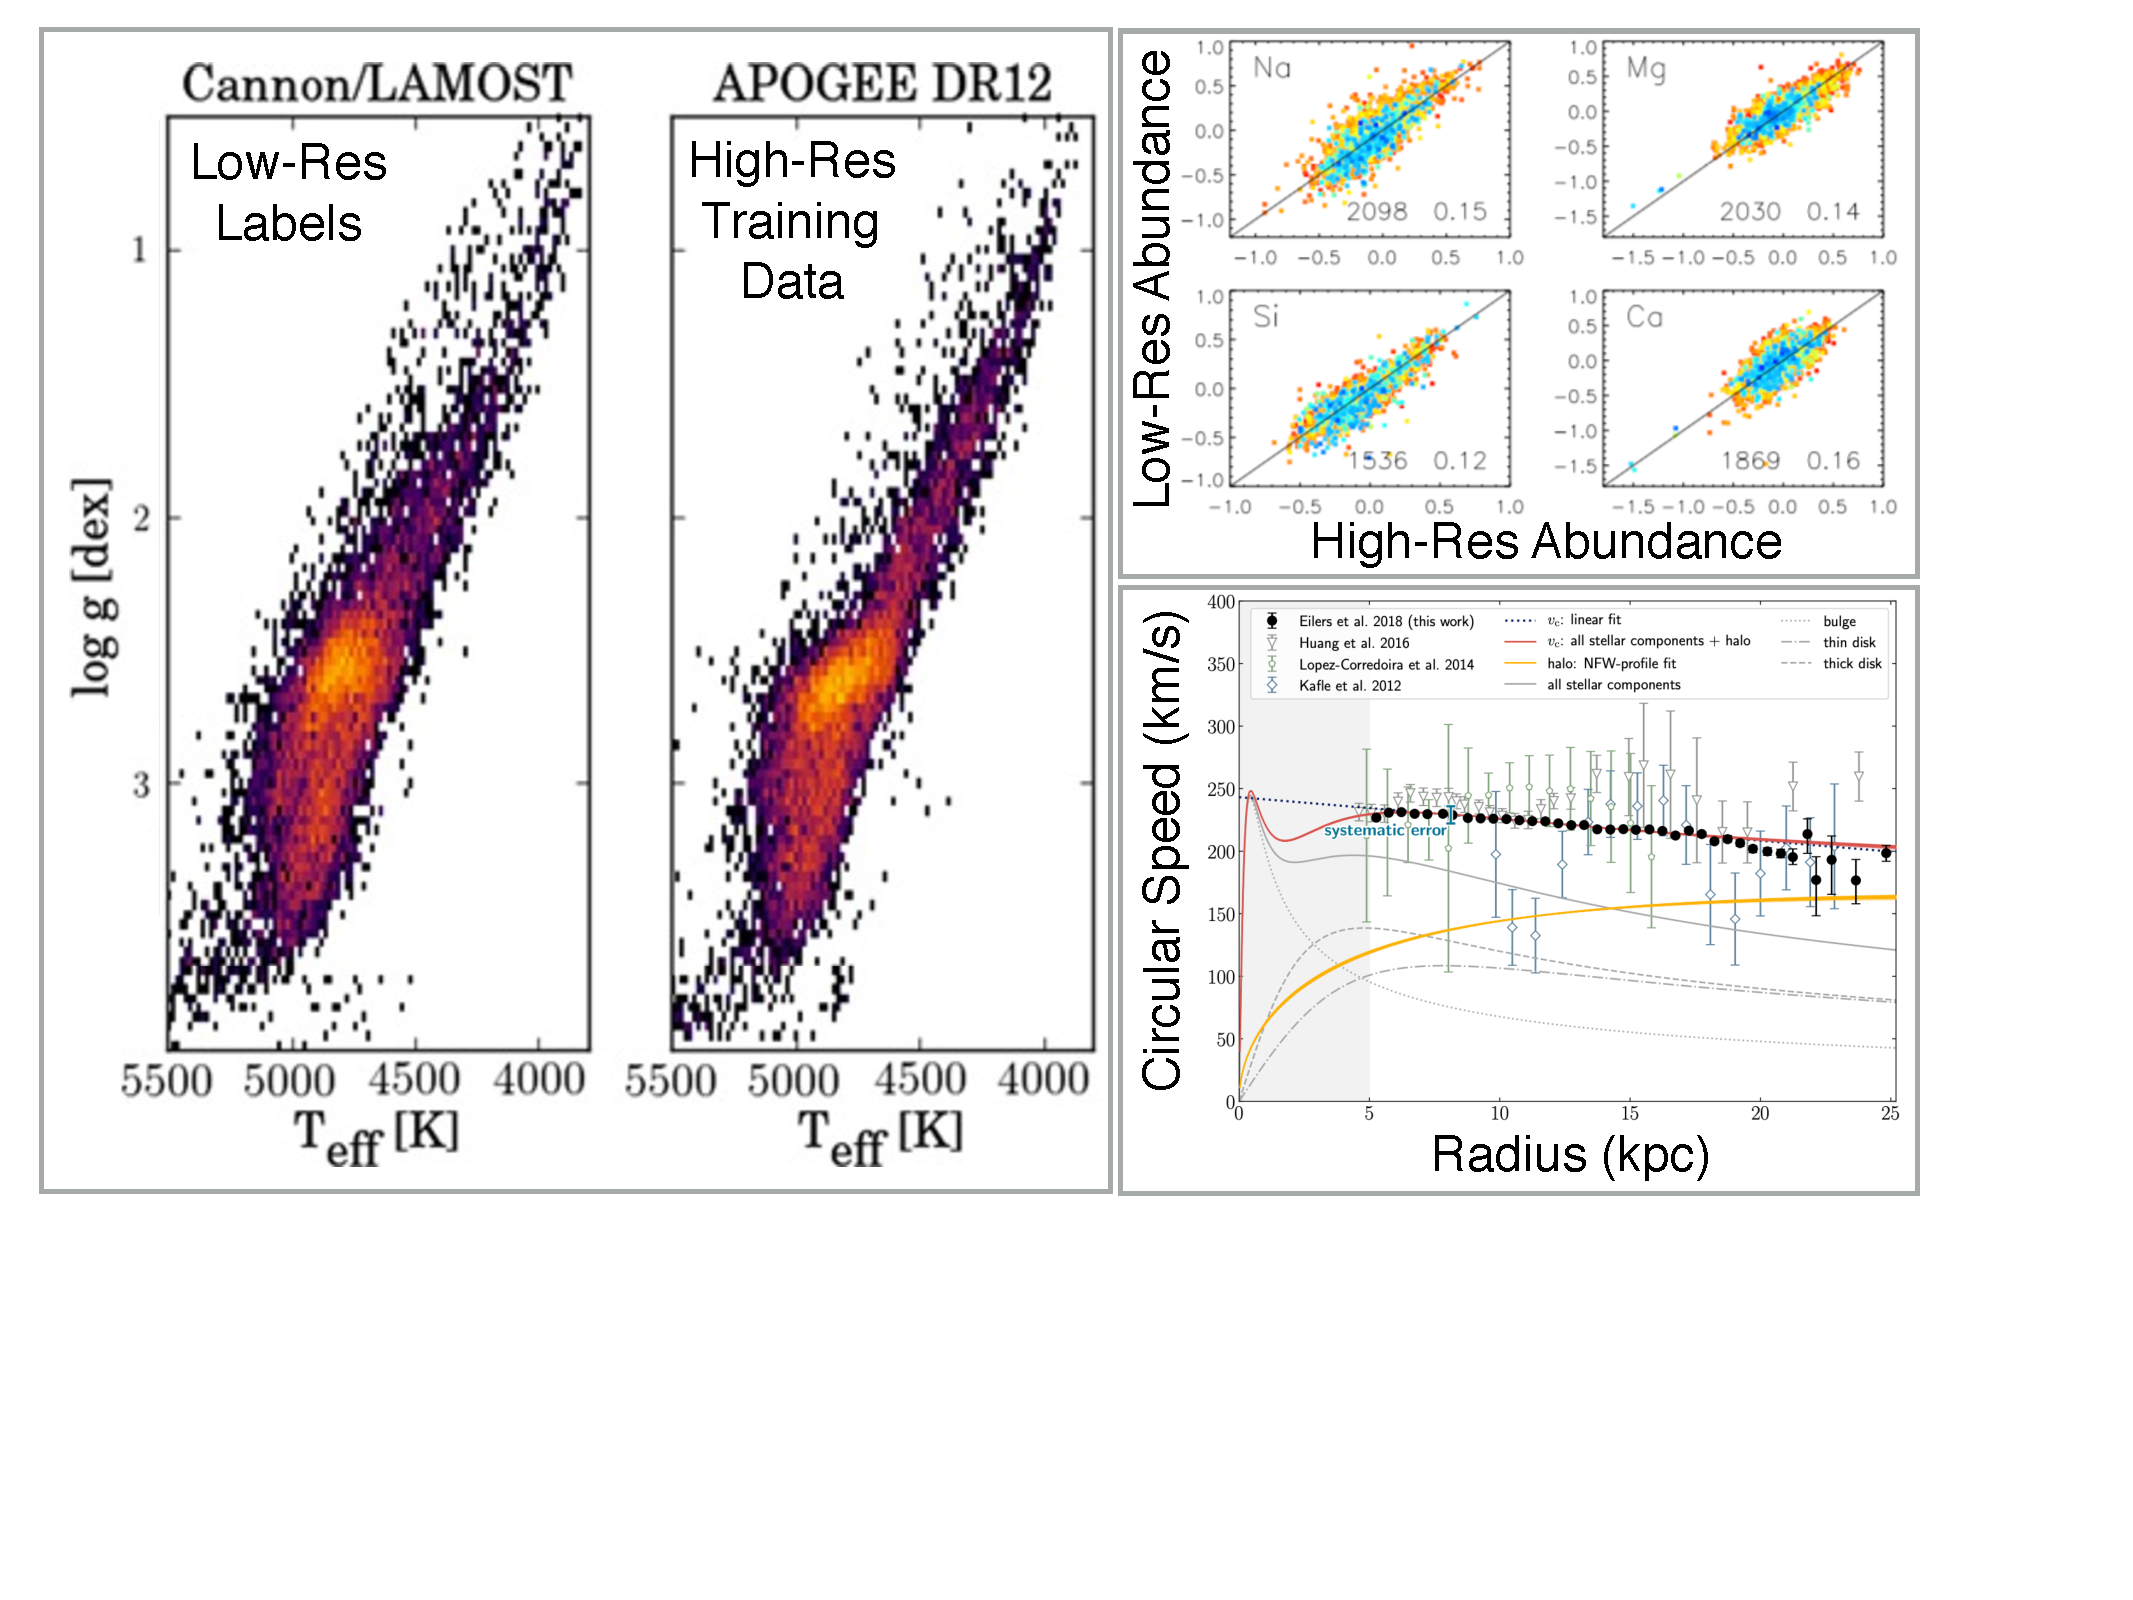
\includegraphics[width=\textwidth]{figs/LGplots.pdf}
%
\caption{{\it Left}: Validation of {\it The Cannon} measurements of
stellar effective temperature, $T_{\rm eff}$, and surface gravity, $\log
g$, using low-resolution LAMOST spectra (left) compared to
high-resolution APOGEE measurements
\citep[right;][]{2017ApJ...836....5H}. {\it Top-right}: Recovery of
elemental abundances from low-resolution LAMOST spectra compared to
high-resolution measurements from GALAH (Xiang et al., in prep).  {\it
Bottom-right}: The circular-speed curve of the Milky Way determined
using a data-driven model that combines stellar parameters determined
from APOGEE spectra with photometry from WISE, 2MASS, and Gaia, yielding
the most precise measurements to date \citep{2019ApJ...871..120E}.}
%
\label{fig:Cannon}
%
\end{figure}
